\section{Основные понятия}
\begin{frame}{Функции переходов по слову в ДКА}
\vspace*{-5pt}
Правила перехода в ДКА $\Aut$ над алфавитом $\Sigma$ и множеством состояний $Q$ определяются функцией $\Sigma\times Q\rar Q$. Если специализировать её по первому аргументу, получится функция $F_{\xi}: Q\to Q$ ($\xi\in\Sigma$). Эту функцию можно продолжить на строки, положив $F_{\xi}\circ F_{\eta} = F_{\eta\xi}$.

\only<1>{\begin{minipage}{0.45\textwidth}
\begin{center}
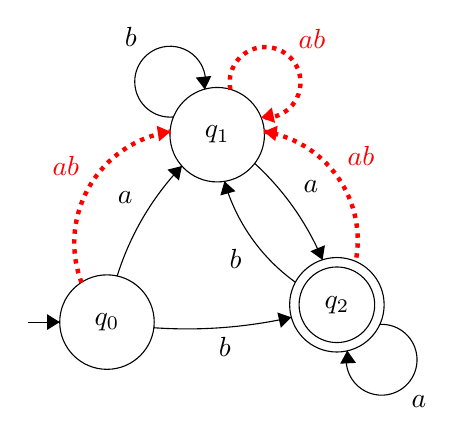
\begin{tikzpicture}[scale=0.2]
\tikzstyle{every node}+=[inner sep=0pt]
\draw [black] (34,-11.1) circle (3);
\draw (34,-11.1) node {$q_1$};
\draw [black] (41.6,-21.9) circle (3);
\draw (41.6,-21.9) node {$q_2$};
\draw [black] (41.6,-21.9) circle (2.4);
\draw [black] (27,-23) circle (3);
\draw (27,-23) node {$q_0$};
\draw [black] (22,-23) -- (24,-23);
\fill [black] (24,-23) -- (23.2,-22.5) -- (23.2,-23.5);
\draw [black] (27.649,-20.075) arc (162.6684:136.40051:17.835);
\fill [black] (31.76,-13.09) -- (30.84,-13.32) -- (31.57,-14.01);
\draw (28.65,-15.1) node [left] {$a$};
\draw [black] (36.377,-12.924) arc (47.5669:22.70148:17.388);
\fill [black] (40.69,-19.05) -- (40.84,-18.12) -- (39.92,-18.5);
\draw (39.46,-14.38) node [right] {$a$};
\draw [black] (38.71,-22.7) arc (-77.36379:-94.01888:30.233);
\fill [black] (38.71,-22.7) -- (37.82,-22.39) -- (38.04,-23.36);
\draw (34.48,-23.91) node [below] {$b$};
\draw [black] (38.97,-20.472) arc (-125.695:-164.03661:11.944);
\fill [black] (34.46,-14.06) -- (34.2,-14.96) -- (35.16,-14.69);
\draw (35.58,-19.01) node [left] {$b$};
\draw [black] (31.232,-9.973) arc (275.56955:-12.43045:2.25);
\draw (28.51,-5.56) node [above] {$b$};
\fill [black] (33.21,-8.22) -- (33.63,-7.37) -- (32.64,-7.47);
\draw [black] (44.317,-23.145) arc (93.11548:-194.88452:2.25);
\draw (46.81,-27.63) node [below] {$a$};
\fill [black] (42.26,-24.81) -- (41.81,-25.64) -- (42.81,-25.59);
\draw [red,dotted,ultra thick] (25.386,-20.497) arc (-159.22321:-261.70788:7.136);
\fill [red] (31.03,-10.91) -- (30.16,-10.53) -- (30.31,-11.52);
\draw (25.26,-13.1) node [left] {\textcolor{red}{$ab$}};
\draw [red,dotted,ultra thick] (36.97,-10.902) arc (81.51001:-11.24163:6.984);
\fill [red] (36.97,-10.9) -- (37.69,-11.51) -- (37.84,-10.53);
\draw (42.25,-12.42) node [right] {\textcolor{red}{$ab$}};
\draw [red,dotted,ultra thick] (34.836,-8.231) arc (191.48955:-96.51045:2.25);
\draw (40.02,-5.64) node [above] {\textcolor{red}{$ab$}};
\fill [red] (36.79,-10.02) -- (37.67,-10.35) -- (37.47,-9.37);
\end{tikzpicture}
\end{center}
\end{minipage}  
\;
\begin{minipage}{0.45\textwidth}
\smallskip
Пусть мы строим функцию переходов по слову $ab$ в автомате $\Aut$. Сначала определим функции $F_a$, $F_b$, определяющие его поведение на буквах $a$ и $b$. Тогда поведение переходов на слове $ab$ получится композицией $F_a$ и $F_b$.
\vspace*{-8pt}
\[\begin{array}{r|ccc}
& q_0 & q_1 & q_2 \\\hline
a & q_1 & q_2 & q_2 \\
b & q_2 & q_1 & q_1 \\
ab & q_1 & q_1 & q_1
\end{array}\]
\end{minipage}}

\only<2>{
\begin{block}{\bf Свойства множества функций переходов ДКА $\Aut$}
\begin{itemize}
\item Существует единичная функция $F_{\empt}$ такая, что $F_{\empt}\circ F_{\xi}=F_{\xi}\circ F_{\empt}=F_{\xi}$.
\item Композиция $\circ$ ассоциативна.
\end{itemize}

Таким образом, функции переходов по словам из $\Sigma^*$ в ДКА $\Aut$ образуют моноид относительно композиции.
\end{block}

\vspace*{-5pt}
\begin{alertblock}{Achtung!}\small
Если ДКА представлен в краткой (trim) форме, некоторые переходы могут вести <<в никуда>>. На самом деле они ведут в (единственное!) состояние-ловушку, существование которого неявно подразумевается. Однако наличие нескольких ловушек в ДКА повлечёт ошибки при построении функции переходов.
\end{alertblock}
}
\end{frame}

\section{Трансформационный моноид} % ClassCard %ClassLength
\begin{frame}{Основные свойства трансформационного моноида}
\vspace*{-6pt}
\begin{block}{\bf Определение}
Трансформационный моноид $\mathcal{M}_{\Aut}$ для ДКА $\Aut$ --- это моноид функций $F_{\xi}$ таких, что $F_{\xi}(q_i)= q_j\iff (q_i\transit{\xi} q_j$ в $\Aut)$. Иначе можно сказать, что трансформационный моноид $\mathcal{M}_{\Aut}$ определяется множеством классов эквивалентности
$\bigl\{w\mid w\in\Sigma^+\bigr\}$ таким, что $w_i = w_j\iff F_{w_i}=F_{w_j}$. 
\end{block} % descriptive documentation 
\begin{itemize}
\item $\mathcal{M}_{\Aut}$ определяется фактормножеством классов эквивалентности и правилами переписывания, задающими эквивалентность. $\empt$ обычно не включается в множество $w_i$.
\item Поскольку множество функций $F_{w_i}$ в случае ДКА конечно, то $\mathcal{M}_{\Aut}$ содержит конечное число классов эквивалентности (верно и обратное: каждый такой моноид определяет некоторый ДКА).
\item Трансмоноид строится для ДКА без ловушек; переход в ловушку обозначается в таблице переходов просто прочерком.
\item Для единообразия записи трансформаций и перестановок в алгебре, в таблице переходов пишут только номера состояний $\Aut$. 
\end{itemize} % overall documentation
\end{frame}

\begin{frame}{Построение трансформационного моноида}
\begin{center}
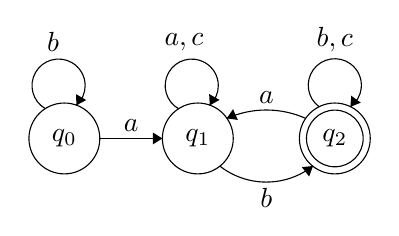
\begin{tikzpicture}[scale=0.15] % the initial automaton placeholder
\tikzstyle{every node}+=[inner sep=0pt]
\draw [black] (24.9,-17.8) circle (3);
\draw (24.9,-17.8) node {$q_0$};
\draw [black] (36.2,-17.8) circle (3);
\draw (36.2,-17.8) node {$q_1$};
\draw [black] (47.8,-17.8) circle (3);
\draw (47.8,-17.8) node {$q_2$};
\draw [black] (47.8,-17.8) circle (2.4);
\draw [black] (27.9,-17.8) -- (33.2,-17.8);
\fill [black] (33.2,-17.8) -- (32.4,-17.3) -- (32.4,-18.3);
\draw (30.55,-17.3) node [above] {$a$};
\draw [black] (23.294,-15.28) arc (240.24286:-47.75714:2.25);
\draw (23.94,-10.5) node [above] {$b$};
\fill [black] (25.92,-14.99) -- (26.75,-14.55) -- (25.89,-14.05);
\draw [black] (34.58,-15.289) arc (240.57068:-47.42932:2.25);
\draw (35.03,-10.45) node [above] {$a,c$};
\fill [black] (37.21,-14.99) -- (38.04,-14.54) -- (37.16,-14.04);
\draw [black] (45.951,-20.128) arc (-51.88249:-128.11751:6.401);
\fill [black] (45.95,-20.13) -- (45.01,-20.23) -- (45.63,-21.02);
\draw (42,-21.99) node [below] {$b$};
\draw [black] (46.477,-15.12) arc (234:-54:2.25);
\draw (47.8,-10.55) node [above] {$b,c$};
\fill [black] (49.12,-15.12) -- (50,-14.77) -- (49.19,-14.18);
\draw [black] (38.655,-16.105) arc (114.1229:65.8771:8.185);
\fill [black] (38.65,-16.1) -- (39.59,-16.23) -- (39.18,-15.32);
\draw (42,-14.89) node [above] {$a$};
\end{tikzpicture}
\end{center}
\only<1>{Oпределим соответствие между буквами и множествами переходов по ним и будем расширять этот список новыми словами в лексикографическом порядке. Если очередное слово задаёт такую же трансформацию, как и уже рассмотренное, порождаем соответствующее правило переписывания.}%overall documentation

\begin{center}
\begin{tabular}{c||c}\hline
 \cellcolor{blue!10}\textbf{Классы эквивалентности} & \cellcolor{blue!10}\textbf{Правила переписывания} \\\hline\hline
 \smallskip
$\begin{array}{r|ccc} % the equivalence class table placeholder
    & 0 & 1 & 2 \\\hline
a   & 1 & 1 & 1 \\
b   & 0 & 2 & 2 \\
c   & - & 1 & 2\only<2>{\\
ab  & 2 & 2 & 2\\
bc & - & 2 & 2 \\
ca & - & 1 & 1 
}
\end{array}$
&
\only<2>{$\begin{array}{cc} % the rewrite rule table placeholder
aa\to a & ac\to a  \\
ba \to a & bb\to b \\
cb\to bc & cc\to c\\ 
abc\to ab & bca\to ca\\
cab\to bc 
\end{array}$}
\end{tabular}
\end{center}
Всего классов эквивалентности: $6$ % the ClassCard placeholder

Максимальная длина факторслова в классах эквивалентности: $2$ % the ClassLength placeholder 
\end{frame}

\section{Синтаксический моноид} % MyhillNerode % IsMinimal
\begin{frame}{Синтаксический моноид}
\vspace*{-7pt}
\begin{block}{}
Определим отношение синтаксической конгруэнтности слов:
\vspace*{-4pt}
\[w_i\sim_{\Lang} w_j\iff \forall x,y(x\,w_i\,y\in\Lang\iff x\,w_j\,y\in\Lang)\]

\vspace*{-4pt}
Синтаксический моноид $\mathcal{M}(\Lang)$ --- это множество его классов эквивалентности относительно $\sim_{\Lang}$. То есть такая полугруппа с единицей над $w\in\Sigma^*$, что $w_i= w_j\iff w_i\sim_{\Lang} w_j$ (равенство здесь понимается в алгебраическом смысле: как возможность преобразовать $w_i$ и $w_j$ к одному и тому же слову).
\end{block} % descriptive documentation

\begin{block}{\bf Лемма}
Синтаксический моноид регулярного языка $\Lang$ совпадает с трансформационным моноидом  минимального ДКА, его распознающего.
\end{block} % descriptive documentation % overall documentation

\begin{alertblock}{}
Синтаксический моноид (так же, как и минимальный ДКА) --- атрибут \textit{языка}, а трансформационный моноид --- атрибут \textit{конкретного ДКА}.
\end{alertblock} % overall documentation
\end{frame}

\begin{frame}{Суффиксная конгруэнтность}
Предшествующие понятия рассматривали  структуру переходов автомата без учёта начальных и конечных состояний\footnote{Хотя неявно они использовались, чтобы удалить недостижимые состояния и состояния-ловушки при подготовке к построению моноида.}. Однако если чуть-чуть специализировать отношение $\sim_{\Lang}$, положив возможные префиксы пустыми, получится отношение эквивалентности, напрямую зависящее от положения стартовых и финальных состояний в минимальном ДКА. % overall documentation

\vspace*{-5pt}
\begin{block}{\bf Определение}
Определим отношение эквивалентности по Нероуду как:
\vspace*{-5pt}
\[w_i\equiv_{\Lang} w_j\iff \forall y(w_i\,y\in\Lang\iff w_j\,y\in\Lang)\]

\end{block} % descriptive documentation

\begin{alertblock}{\bf Achtung!}
Обозначение $\sim_{\Lang}$ может использоваться в литературе как в смысле синтаксической конгруэнции, так и в смысле эквивалентности по Нероуду. Лучше дополнительно уточнить.
\end{alertblock} % overall documentation
\end{frame}

% overall documentation - frame
\begin{frame}{Критерий регулярности языка}

\begin{block}{\bf Теорема Майхилла--Нероуда}
Язык $\Lang$ регулярен тогда и только тогда, когда множество классов эквивалентности по $\equiv_{\Lang}$ конечно.
\end{block}
{$\logimpl:$ Пусть $\Lang$ регулярен. Тогда он порождается некоторым DFA $\Aut$ с конечным числом состояний $N$. Значит, множество $\bigl\lbrace{}q_i\mid q_0\transit{w} q_i\bigr\rbrace{}$ конечно, а для каждых двух $w_1$, $w_2$ таких, что $q_0\transit{w_1} q_i$ и $q_0\transit{w_2} q_i$, выполняется $w_1\equiv_{\Lang} w_2$.}

\medskip
{$\Leftarrow:$ Пусть все слова в $\Sigma^*$ принадлежат $N$ классам эквивалентности $A_1$,\dots, $A_n$ по $\equiv_{\Lang}$. Построим по ним DFA $\Aut$, распознающий $\Lang$. Классы $A_i$ сопоставим состояниям:
\begin{itemize}
\item Начальным объявим класс эквивалентности $A_0$ такой, что $\empt\in A_0$.
\item Конечными объявим такие $A_j$, что $\forall w\in A_j (w\in\Lang)$.
\item Если $w\in A_i$, $w\,a_k\in A_j$, тогда добавляем в $\delta$ правило $\langle A_i, a_k, A_j\rangle$.
\end{itemize}}
\end{frame}

% overall documentation - frame
\begin{frame}{Трансформационный моноид и отношение $\equiv_{\Lang}$}
\begin{itemize}
\item Классы эквивалентности по Майхиллу--Нероуду можно извлечь из трансформационного моноида минимального ДКА для языка $\Lang$: они являются подмножеством факторслов, которые переводят стартовое состояние в какое-то другое (непустое) состояние.
\item Для каждой пары таких факторслов $w_i$ и $w_j$, переводящих стартовое состояние в разные состояния $q_i$ и $q_j$, в синтаксическом моноиде обязательно найдётся различающий суффикс (т.е. класс эквивалентности $u$ такой, что $w_i\,u\in\Lang\logand w_j\,u\not\in\Lang$, либо наоборот).
\item Если в ДКА существует ловушка (возможно, неявная), то в трансформационном моноиде найдётся класс эквивалентности, переводящий в неё стартовое состояние. Таких классов может быть несколько, но с точки зрения эквивалентности по Майхиллу--Нероуду, они не различаются.  
\end{itemize}

\end{frame}

\begin{frame}{Классы эквивалентности по Майхиллу--Нероуду}
\vspace*{-5pt}
\begin{center}
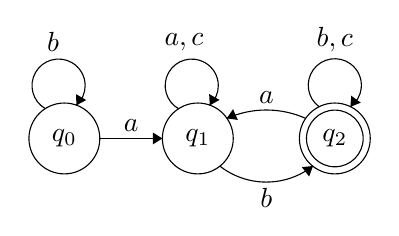
\begin{tikzpicture}[scale=0.15] % the initial automaton placeholder
\tikzstyle{every node}+=[inner sep=0pt]
\draw [black] (24.9,-17.8) circle (3);
\draw (24.9,-17.8) node {$q_0$};
\draw [black] (36.2,-17.8) circle (3);
\draw (36.2,-17.8) node {$q_1$};
\draw [black] (47.8,-17.8) circle (3);
\draw (47.8,-17.8) node {$q_2$};
\draw [black] (47.8,-17.8) circle (2.4);
\draw [black] (27.9,-17.8) -- (33.2,-17.8);
\fill [black] (33.2,-17.8) -- (32.4,-17.3) -- (32.4,-18.3);
\draw (30.55,-17.3) node [above] {$a$};
\draw [black] (23.294,-15.28) arc (240.24286:-47.75714:2.25);
\draw (23.94,-10.5) node [above] {$b$};
\fill [black] (25.92,-14.99) -- (26.75,-14.55) -- (25.89,-14.05);
\draw [black] (34.58,-15.289) arc (240.57068:-47.42932:2.25);
\draw (35.03,-10.45) node [above] {$a,c$};
\fill [black] (37.21,-14.99) -- (38.04,-14.54) -- (37.16,-14.04);
\draw [black] (45.951,-20.128) arc (-51.88249:-128.11751:6.401);
\fill [black] (45.95,-20.13) -- (45.01,-20.23) -- (45.63,-21.02);
\draw (42,-21.99) node [below] {$b$};
\draw [black] (46.477,-15.12) arc (234:-54:2.25);
\draw (47.8,-10.55) node [above] {$b,c$};
\fill [black] (49.12,-15.12) -- (50,-14.77) -- (49.19,-14.18);
\draw [black] (38.655,-16.105) arc (114.1229:65.8771:8.185);
\fill [black] (38.65,-16.1) -- (39.59,-16.23) -- (39.18,-15.32);
\draw (42,-14.89) node [above] {$a$};
\end{tikzpicture}
\end{center}
\vspace*{-5pt}
\small{Включим в число факторслов $\empt$ и выделим по одному факторслову для каждого состояния $q_i$, переводящему стартовое слово в $q_i$. Для каждого из них определим множество суффиксов, которые оставляют слова этих классов в языке. После этого достаточно собрать вместе все суффиксы и префиксы и выкинуть из полученной таблицы дубли столбцов.} % overall documentation

\begin{center}
\begin{tabular}{c||c}\hline
 \cellcolor{blue!10}\textbf{Факторслова--префиксы} & \cellcolor{blue!10}\textbf{Таблица классов эквивалентности} \\\hline\hline
 \smallskip
$\begin{array}{r|c|c} % the equivalence class table placeholder
\text{префикс}    & 0\to ? &\text{суффиксы} \\\hline
{\empt}   & 0 &  ab\\
{a}   &  1 & b, ab\\
{ab}  & 2 & \empt, b, ab
\end{array}$
&
$\begin{array}{r|ccc} % the MyhillNerode table placeholder
& \empt & b & ab \\\hline
\empt & - & - & +  \\
a & - & + & + \\
ab & + & + & +
\end{array}$
\end{tabular}
\end{center}
Всего классов эквивалентности по Майхиллу--Нероуду: $3$ % the MyhillNerode placeholder

\end{frame}